\section{Исследовательская часть}

\noindent
\hspace{1.25cm}
В данном разделе сравниваются временные характеристики построения деформированной трубки в зависимости от количества сечений и количества точек в каждом сечении. 

\noindent
\hspace{1.25cm}
Замеры для нахождения зависимости времени от количества сечений проводились для трубок с количеством сечений от 10 до 50. В каждом сечении было от 25 точек. Замеры для нахождения зависимости времени от количества точек проводились для трубок с количеством точек от 10 до 100. В трубке было 20 сечений. Деформация происходила по центру трубки с одинаковым радиусом влияния. Все замеры проводились 100 раз и в таблицу заносилось среднее арифметическое значение времени.

\subsection{Технические характеристики}

\noindent
\hspace{1.25cm}
Тестирование программы проводилось на устройстве с операционной системой Windows 11, оснащенном процессором Intel Core i7-1260p, оперативной памятью объемом 16 Гб и видеокартой Intel Iris Xe Graphics. Во время тестирования, компьютер был подключен к сети питания и не использовался для других задач.

\subsection{Замеры времени выполнения деформации в зависимости от количества сечений}

\begin{table}[H]
    \captionsetup{justification=raggedright, singlelinecheck=false}
    \caption{Зависимость времени построения деформированной трубки от количества сечений (в миллисекундах)}
    \label{tab:time_sections}
    \begin{tabularx}{\textwidth}{|>{\centering\arraybackslash}X|>{\centering\arraybackslash}X|}
        \hline
        \textbf{Количество сечений} & 
        \textbf{Время построения (мс)} \\ \hline
        10 & 981.263 \\ \hline
        20 & 1196.770 \\ \hline
        30 & 1342.660 \\ \hline
        40 & 1587.540 \\ \hline
        50 & 1845.920 \\ \hline
    \end{tabularx}
\end{table}

\begin{figure}[H]
\centering
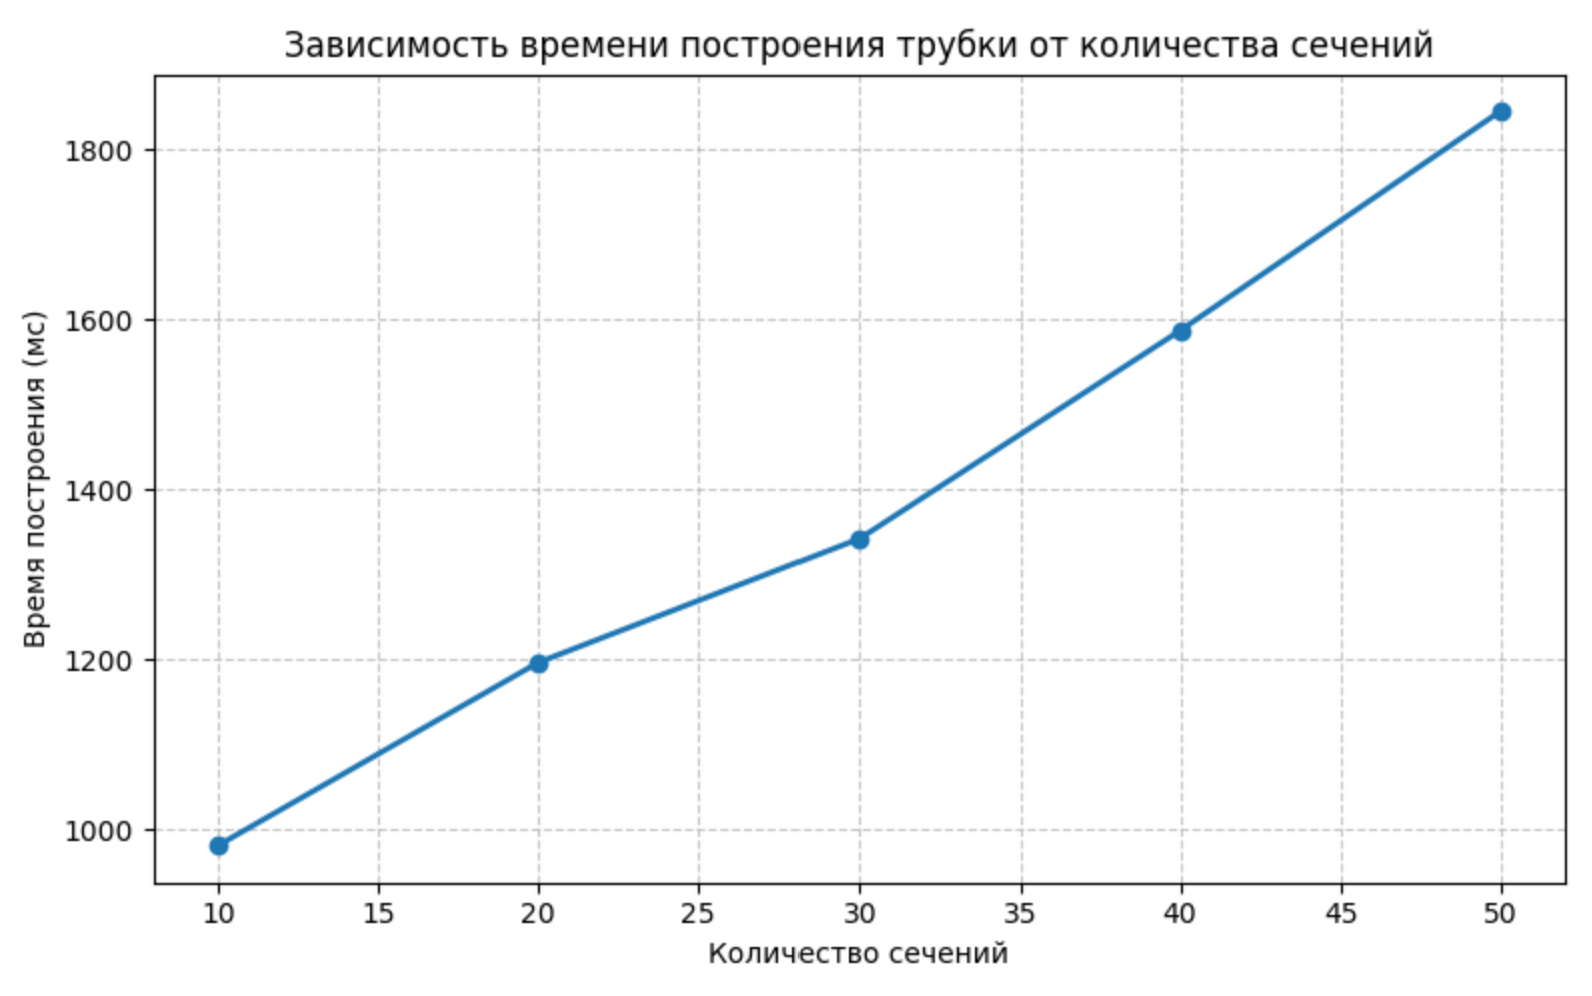
\includegraphics[width=0.8\textwidth]{img/graf_1.png}
\caption{График зависимости времени построения деформированной трубки от количества сечений}
\label{fig:geom_base_same}
\end{figure}

\subsection{Замеры времени выполнения деформации в зависимости от количества точек}

\begin{table}[h]
    \captionsetup{justification=raggedright, singlelinecheck=false}
    \caption{Зависимость времени построения деформированной трубки от количества точек в сечении (в миллисекундах)}
    \label{tab:time_points}
    \begin{tabularx}{\textwidth}{|>{\centering\arraybackslash}X|>{\centering\arraybackslash}X|}
        \hline
        \textbf{Количество точек} & \textbf{Время построения (мс)} \\ \hline
        10  & 992.191 \\ 
        25  & 1196.770 \\  
        50  & 1345.230 \\ 
        75  & 1462.880 \\ 
        100 & 1578.440 \\ 
        \hline
    \end{tabularx}
\end{table}

\begin{figure}[H]
\centering
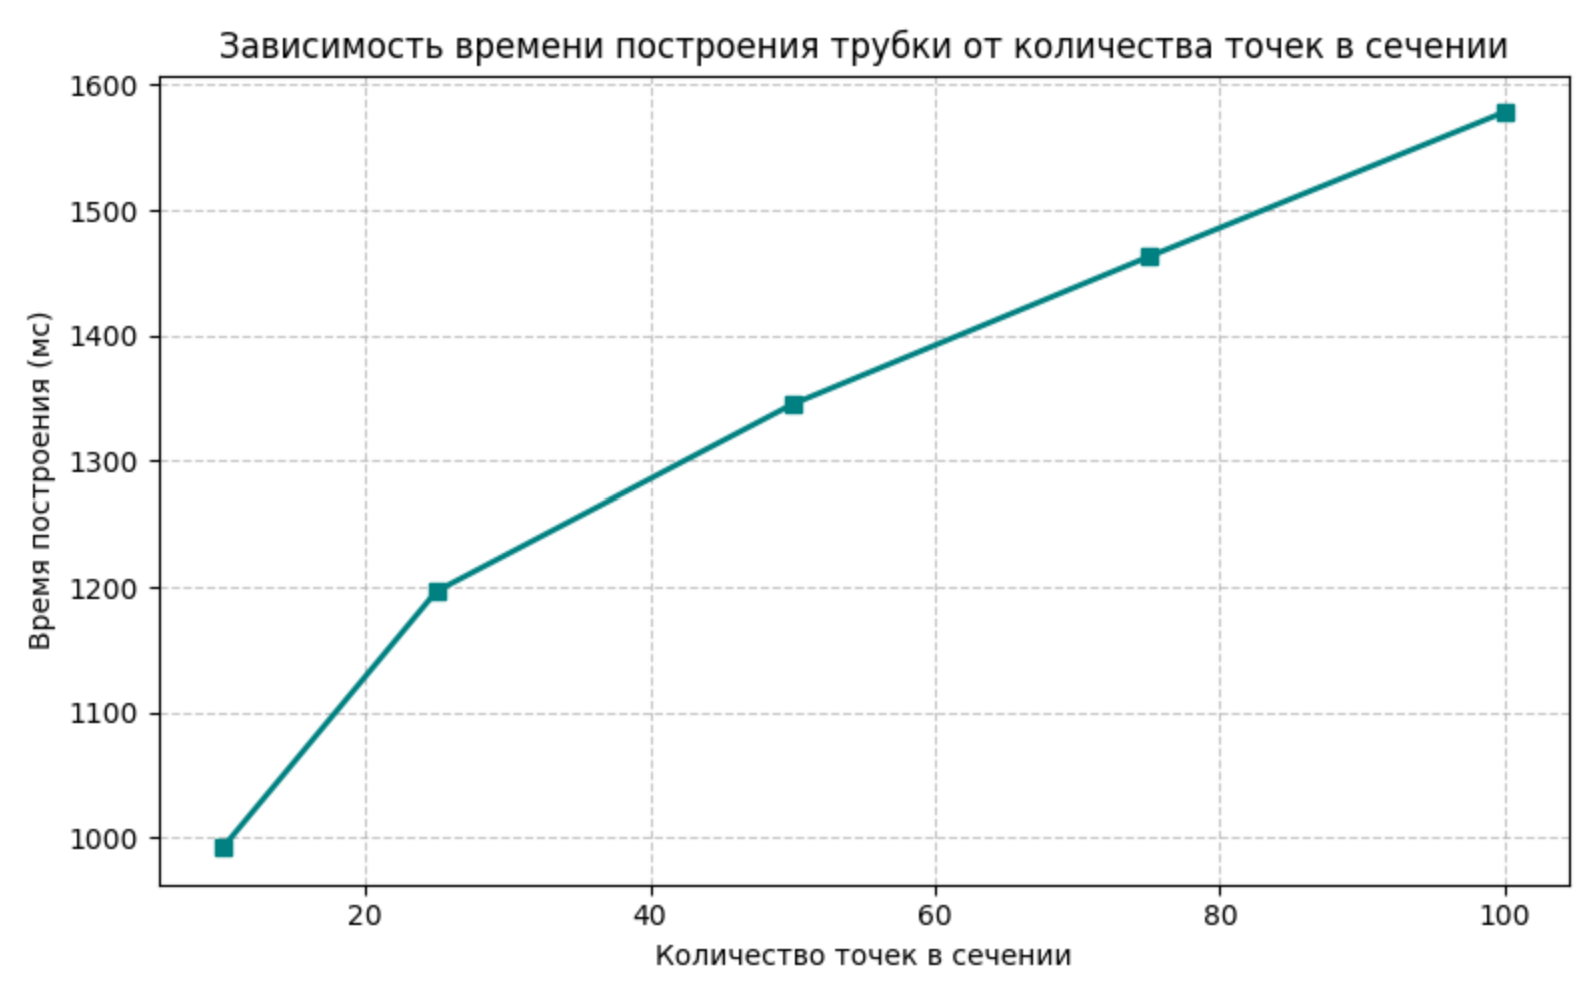
\includegraphics[width=0.8\textwidth]{img/graf_2.png}
\caption{График зависимости времени построения деформированной трубки от количества точек}
\label{fig:geom_base_dif}
\end{figure}

\subsection{Вывод}

\noindent
\hspace{1.25cm}
В данном разделе были сравнены временные характеристики построения деформированной трубки в зависимости от количества сечений и количества точек в каждом сечении. 

\noindent
\hspace{1.25cm}
Полученные результаты показывают, что время построения деформированной трубки линейно возрастает как с увеличением количества сечений, так и с ростом числа точек в каждом сечении.